\FloatBarrier
\section{The Gross-Neveu-Yukawa model at finite \texorpdfstring{$N$}{N}}\label{sec:gnyFiniteN}
\begin{disclaimer}
	In this section we mainly follow the discussion of results presented in Sec. VI of \ccite{Stoll:2021ori}.
	
	The plots of \ccite{Stoll:2021ori} and the majority of underlying numerical data were produced by N. Zorbach.
	Selected results have been cross-checked by J. Stoll, A. Koenigstein, and me.
	The single thread wall time on various consumer processors for the numeric results of \ccite{Stoll:2021ori} is around 80 days, with most of it spend on the 
	computation of the phase diagram~\ref{fig:phase_boundaries}.
\end{disclaimer}
After our discussions in the infinite-$N$ limit of \cref{sec:gnInfHomo,sec:gnInfInhomo} it is time to use our adapted \cfd{} \frg{} formalism of \cref{sec:gny_frg} to study the \gnym{} at finite $N$.
To this end we will first give a brief overview of the literature concerning the \gnyBm{} at finite $N$ in \cref{subsec:z2breaking}.
Even though there seem to be a lot of indications and notions, that there should not be any symmetry breaking in the \gnyBm{} at finite $N$ and $T>0$, the question is still unsettled and will be at the heart of our research in this section.

So far we have not specified a specific \uv{} initial condition for our \lpa{} flow \cref{eq:pdeq-U}/\eqref{eq:pdeq-u} of the \gnym{}.
In \cref{subsec:UUV} we will continue the discussion of \cref{paragraph:GNbGNGNY} by incorporating our findings/rediscoveries of \cref{subsec:GNUvac} to construct a \uv{} initial condition viable for flows at finite and infinite $N$, which is based on the notion of asymptotic freedom.
As a first step we will use this \ic{} and our \cfd{} numerics to recover the renormalized, infinite-$N$ phase diagram \cref{fig:GNlargeN_PD}.

We conclude this section with our \frg{} study of the \gnym{} at finite $N$ in \cref{subsec:gnyFiniteNresults}.
We employ our \cfd{} numerics and perspective to discuss the role of fermionic and bosonic fluctuations in \frg{} flows at zero and non-zero temperature and chemical potential.
The main result of our explicit computations, summarized by the phase diagram~\ref{fig:phase_boundaries} of the \gnym{} at $N=2$, is that bosonic thermal fluctuations vaporize the chiral condensate at any finite $N$ and $T>0$.
This finding is in line with the vague consensus of arguments in \cref{subsec:z2breaking}, which predict such an outcome but usually are not based on explicit computations at finite $N$.
The \cfd{} perspective of \frg{} flows developed in \cref{chap:zeroONSU2} allows for a unique and detailed understanding of the role the different fluctuations at finite $N$.

\subsection{To break or not to break -- \texorpdfstring{$\mathds{Z}_2$}{Z2} symmetry at finite \texorpdfstring{$N$}{N}}\label{subsec:z2breaking}
\begin{disclaimer}
	This subsection has been copied from Sec.~I.B of \nbccite{Stoll:2021ori} with only small adaptations to the presentation in this thesis.
	While I am the author of a first draft of this subsection, I do not claim sole authorship, since it went through iterations during the preparation of the manuscript for \ccite{Stoll:2021ori}.
\end{disclaimer}
The big question that immediately comes to mind if one relaxes the infinite-$N$ limit and studies the \gnm{} for finite $N$ is, if \ssb{} and condensation still takes place, especially when medium effects (non-zero $\mu$ and/or $T$) are included.

At first sight, it seems as if already the \acrrepeat{cmwh} theorem~\cite{Mermin:1966,Hohenberg:1967,Coleman:1973ci} forbids the formation of a condensate at non-zero temperatures. Though, the theorem strongly relies on the presence of massless Nambu-Goldstone bosons~\cite{Nambu:1960tm,Goldstone:1961eq,Goldstone:1962es}, which are only included in extensions of the \gnm{}, \eg{}, the chiral \gnm{}~\cite{Schon:2000qy,Basar:2009fg,Furuya:1982fh} with continuous chiral symmetry or other related models~\cite{Witten:1978qu,Rosenstein:1990nm}. We therefore believe that one should exercise caution, when arguing directly with this theorem.

Nevertheless, a qualitative argumentation was put forward already by L.~D.~Landau in 1950~\cite{Landau:1980mil}, which should in principle forbid also discrete chiral symmetry breaking in one-spatial dimension at non-zero temperature. L.~D.~Landau and E.~M.~Lifshitz argue in Chap.~163 of \ccite{Landau:1980mil} that for systems in one dimension of infinite extent only one phase can exist at $T>0$, since coexistence of more than one phase is energetically disfavored. To be concrete, they considered a bistable system in one dimension of infinite extent at non-zero temperature with $n$ interfaces between the two possible phases per length $L$ and showed that the thermodynamic potential of the system can be decreased by increasing the concentration of interfaces $n/L$, which is directly related to the entropy, assuming a finite interface energy. Thus the system breaks down into a macroscopic number of domains, which rendered macroscopic phase coexistence at non-zero temperature impossible. Landau's argument can be applied to a broad range of effectively one-dimensional systems including the Ising model in one spatial dimension~\cite{Ising:1925em} at $T \neq 0$, which is always in its \ZII{}-symmetric phase, \cf{} \ccite{ZinnJustin:2002ru,Rosenstein:1990nm}. A dedicated discussion of Landau's argument in the context of one-dimensional systems can be found in \ccite{Theodorakopoulos:2006}.

 In their study~\cite{Dashen:1974xz} of the \gnm{} based on a large-$N$ expansion R.~F.~Dashen, S.~Ma, and R.~Rajaraman were able to confirm Landau's argument, see also \ccite{Barducci:1994cb}. They found no \ssb{} for any small but non-zero temperature and finite $N$. Using in parts heuristic arguments, they showed that the entropic gain of a field configuration of alternating kinks is large enough at finite $N$ and $1/T$ to be energetically preferred over a homogeneous configuration\footnote{Homogeneous and inhomogeneous field configurations in this context refer to the configurations used to evaluate the partition function in a saddle-point approximation, see \ccite{Dashen:1974xz} for details on their computation, and they are not to be confused with homogeneous and inhomogeneous classical/mean field configurations $\langle \Fpsib\,\Fpsi \rangle(x)$ discussed in the previous \cref{paragraph:GN_pheno}.}. Those field configurations alternating in kinks have a vanishing chiral condensate $\langle \Fpsib\,\Fpsi  \rangle = 0$. In the infinite-$N$-limit (mean-field), the energy per kink becomes infinite and consequently the density of kinks approaches zero realizing a homogeneous field configuration compatible with $\langle  \Fpsib\,\Fpsi  \rangle > 0$ allowing for \ssb{}. This is no contradiction to Landau's argument since the latter only holds assuming finite interface energies~\cite{Landau:1980mil,Theodorakopoulos:2006}. Although R.~F.~Dashen, S.~Ma, and R.~Rajaraman argue that $T_\mathrm{C} = 0$ at finite $N$, they do not discuss the situation for $T = 0$ and $\mu \geq 0$ for finite $N$ in \ccite{Dashen:1974xz}.

Another discussion on the absence of symmetry breaking in one-spatial dimension at non-zero $T$ can be found in \ccite{Witten:1978qu} by E.~Witten, which discusses the absence of a phase with spontaneous symmetry breaking and long-range order in accordance with the \cmwhTheoremWithRefs{} and the related possibility for a phase of Berezinski-Kosterlitz-Thouless type~\cite{Berezinsky:1970fr,Kosterlitz:1973xp} with quasi long-range order for the $\mathrm{SU}(N)$ Thirring model~\cite{Thirring:1958in,Witten:1978qu}.

Other authors, \eg{}, U.~Wolff~\cite{Wolff:1985av}, argue based on the duality of the spatial and Euclidean time direction in \dimPlus{1}{1} dimensions for $T>0$ and $\mu=0$: The thermal \gnm{} in \dimPlus{1}{1} dimensions is equivalent to a \qft{} with a finite spatial volume (but infinite Euclidean time-direction) and hence no \ssb{} takes place since it is canonically considered as an effect only present in systems with infinite volumes, see, \eg{}, \ccite{Weinberg:1996kr}. While this reasoning \dash{} the general absence of \ssb{} in finite systems \dash{} might strictly speaking be sound, sufficiently large volumes, the inclusion of small (possibly infinitesimal) explicit symmetry breaking, or subtleties of the thermodynamic and/or infinite volume limit, \cf{}\ \ccite{Landsman:2013aoa}, can lead to signatures reminiscent of \ssb{}.

Indeed, only recently some of our colleagues and collaborators found some indications via numerical lattice Monte-Carlo simulations~\cite{Pannullo:2019bfn,Pannullo:2019prx,Lenz:2020bxk,Lenz:2020cuv}, that some (inhomogeneous) condensation phenomena in the massless \bgnm{} at finite $N$ and non-zero $\mu$ and $T$ still seem to be present. Similar results were already found in earlier lattice Monte-Carlo studies~\cite{Cohen:1981qz,Cohen:1983nr,Karsch:1986hm} at finite $N$. However, in all of these works, the above arguments by Landau \etal{}\ against condensation at non-zero $T$ could neither be completely ruled out nor be confirmed. In fact, most of the results suffer from the facts that proper continuum and infinite volume extrapolations were not performed. Consequently finite volume effects and discretization artifacts limit the predictive power of those results for the continuum theory in an infinite volume. The finite sized spatial domain (and the related \bcs{}) might have prevented a sufficient resolution of long-range fluctuations, which are however of uttermost importance for condensation and in this context especially vaporization phenomena in low-dimensional systems.

Recent lattice results presented in \ccite{Pannullo:2019bfn,Pannullo:2019prx,Lenz:2020bxk,Lenz:2020cuv} have sparked further lattice studies of four-Fermi models in $1 + 1$ dimensions: We are aware of these parallel developments and computations using lattice Monte Carlo simulations in the \gnm{} and related models (especially the chiral \gnm{}) in \ccite{Mandl2021,Nonaka2021}, which are however not completed yet and therefore omitted in the following discussion. For the chiral \gnm{}, we expect some interesting dynamics at finite $N$ due to competing effects from the \cmwhTheorem{} and a $U ( 1 )_\mathrm{A}$ anomaly~\cite{Furuya:1982fh}.\bigskip

All of this lead us to the idea to study the phenomenon of \ZII{} symmetry breaking and/or restoration in the \gnm{} at finite $N$, $T\geq0$, and also $\mu\geq0$ but in an infinite spatial volume within a different framework \dash{} namely within our \cfd{} frame work for \frg{} flow equations.\footnote{After completing \ccite{Stoll:2021ori}, we became aware of \ccite{Blaizot:2002nh}, where next-to-leading order corrections of the $\tfrac{1}{N}$-expansion to the effective potential of the \gnm{} were calculated. Finding that this expansion breaks down in the vicinity of mean-field critical temperature $T_\mathrm{C}$ the authors also suggest to analyze the \gnm{} within the \frg{} framework, which is the main focus of this section and one main purpose of this whole chapter. We thank J.~Braun for drawing our attention to this interesting publication.} We wanted to find out, if it is possible to (numerically) confirm the arguments by Landau \etal{}\ against symmetry breaking in the \gnm{} or if there are some other competing effects, which are not captured in the aforementioned mostly qualitative/heuristic discussions, that allow for symmetry breaking or some long-range ordering. 
	
\subsection{UV initial condition for FRG flows at variable \texorpdfstring{$N$}{N}}\label{subsec:UUV}
\begin{disclaimer}
	This subsection is based on Secs.~V.D and E of \nbccite{Koenigstein:2021llr}.
\end{disclaimer}
We again turn to the \uv{} \ic{} for the effective potential and continue the discussion of \cref{paragraph:GNbGNGNY}.
For practical calculations within the \frg{} framework, where the flow is not integrable analytically, we can not initialize the \frg{} flow directly at $\Lambda = \infty$.
But rather we have to choose a sufficiently large and but finite $\Lambda$ to specify the initial values for the flow via $\bar{\Gamma}_\Lambda [ \chi ] = \mathcal{S} [ \chi ]$.
For a general discussion in the context of \rgcy{} we refer to \cref{subsec:RGconsistency} and our specific, explicit discussion of the issue in zero dimensions in \cref{paragraph:ONRGconsistency}.\bigskip

From the previous discussion in \cref{subsec:GNUvac}, it is obvious, how to specify the \ic{} for a numeric solution of \cref{eq:pdeq-U-MF} or rather \cref{eq:pdeq-u} with $Q ( t, \partial_\sigma u) = 0$, \ie{}, in the mean-field approximation:

In our discussion on asymptotic freedom, we were able to eliminate $g^2$ from the \ic{} \eqref{eq:initial_potential} in favor of the \uv{} scale $\Lambda$ and the combination $\Delta_0\equiv h \sigma_0$.
Hence, we can simply use \cref{eq:initial-condition} as the initial potential at some large scale $\Lambda$.
Initializing the (numeric) mean-field version of the \frg{} flow \eqref{eq:pdeq-u} with the $\sigma$-derivative of \eqref{eq:initial-condition} and an arbitrary value for $h$ at some scale $\Lambda \ggg h$, one always finds that the \ir{} minimum in vacuum is located at $\sigma_0$. 
Consequently and \wlogA{} we can rescale all dimensionful quantities in terms of $h$ and express the dimensionless field space variable $\sigma$ in multiples of $\sigma_0$.
On the level of the equations, this amounts to setting $\sigma_0 = 1$ and $h = 1$.
Other choices for $h$ and $\sigma_0$ correspond to different renormalization conditions, but all results are unique and can be transformed into each other via simple rescaling \dash{} as already mentioned.
However, we still have to ensure that other \ir{} observables do not depend on the \uv{} scale $\Lambda$, which is realized by choosing $\Lambda$ much larger than all internal and external model scales. 
This checked numerically in the \customref{paragraph:numeric_consistency_check_mean-field}{following paragraph} discussing \cref{fig:MF_consistency_check}.\bigskip

Including bosonic quantum fluctuations, it is less obvious, how to choose the \ic{} for the \frg{} flow, that means how to choose a meaningful value for $\frac{h^2}{g^2}$ in \cref{eq:uv-initial}. When performing calculations at finite $N$, each individual choice of $N$ represents a single model on its own. 
Hence, even if there is symmetry breaking for the vacuum flow equation \eqref{eq:vacuum_limit_flow_equation} including bosonic quantum fluctuations, the \ir{} physics for different $N$ is not necessarily directly comparable.
Thus, setting a unique renormalization condition for all $N$ in the \ir{}, like fixing the position of the \ir{} minimum and/or the \ir{} curvature mass by tuning the various \uv{} \ics{}, is \dash{} to the best of our knowledge \dash{} not useful.

We think that it is natural to use exactly the same \ic{} for all \frg{} flows, namely \cref{eq:initial-condition}, with and without bosons and to fix the renormalization condition for the bosonic \frg{} flows in the \uv{}.
This might be counter-intuitive, because in a lot of \frg{} studies for effective models of strongly correlated systems, the physics is fixed in the \ir{} and the \uv{} \ic{} is tuned, in such a way that the \frg{} flow ends up with an \ir{} effective action having observables compatible with desired numerical values. 
We are however using the \gnm{} in our studies with the same top-down approach, used in the \frg{} studies of \qcd{}, discussed in \cref{subsec:chiralLEFT}.
We make use of asymptotic freedom and \rgcy{} to fix our initial condition and associated \uv{} initial scale $\Lambda$ in the following way.\bigskip

Using the same \uv{} \ic{} for all finite and infinite $N$ allows for a direct comparison of calculations at different $N$.
This is the case, because the $\tfrac{1}{N}$-rescaled \uv{} potential \eqref{eq:initial-condition} always describes a theory of $N$ asymptotically free fermions and a \sigmaMode{} that decouples from the system at the \uv{} initial scale.
Choosing $\Lambda \ggg h$ naturally leads to a large curvature mass $\partial_\sigma^2 U ( t, \sigma )$ and suppression of fluctuations of the \sigmaMode{} in the \uv{}, which can be directly seen in \cref{eq:initial-condition}.
On a formal level this can be seen by inspecting the fluid-dynamic formulation of the \frg{} flow equation \eqref{eq:pdeq-u} and especially its bosonic contribution in terms of a highly non-linear diffusion equation \eqref{eq:heat_equation_analogy}. One finds that the large curvature mass $\partial_\sigma^2 U ( t, \sigma )= \partial_\sigma u ( t, \sigma )$ in the propagators $\tfrac{1}{E_\sigma}$ yields a small diffusion coefficient $\alpha ( t, \partial_\sigma u )$ and therefore a suppression of the diffusion along field space \dash{} the bosonic contribution to the \frg{} flow.

Though, the more drastic argument, why bosonic fluctuations are actually totally absent in the \uv{}, is a fundamental property of all diffusion equations of type $\partial_t u ( t, \sigma ) \propto \partial_\sigma^2 u ( t, \sigma )$. Independent of the finite diffusion coefficient the term $\partial_\sigma^2 u( t, \sigma ) $ vanishes exactly for spatially linear $u ( t, \sigma ) \propto \sigma$ and the diffusion and dynamics stops, \cf{} \cref{paragraph:HE} and especially the discussion surrounding \cref{eq:heICS1asymp} as an equilibrium solution to the \heq{} with Dirichlet \bcs{}.
In the context of this work, it follows from the quadratic \uv{} potential \eqref{eq:uv-initial} that $u ( 0, \sigma ) \propto \sigma$ and consequently the contribution from the \sigmaMode{} to the \frg{} flow vanishes exactly.
Bosonic fluctuations will be suppressed as long as the fermionic source/sink contributions to the \frg{} flow do not alter the linear shape of $u ( t, \sigma )$, which is approximately the case until $k^2 ( t ) \approx ( h \sigma )^2$ for small $\sigma$. 
We conclude that the \frg{} trajectories in theory space for \frg{} flows including fermions and bosons at finite $N$ will approximately follow the mean-field \frg{} trajectories for infinite $N$, as long as the \uv{} initial potential is quadratic in $\sigma$.
This behavior is indeed observed in our numeric computations in \cref{subsec:gnyFiniteNresults}.

It also gives merit to our choice of setting $Z_\varphi ( t=0 ) = 1$ in the \uv{} and we expect to resemble the dynamics of the \gnm{} with the \gnym{} in \lpa{} to a certain extent.
Even though $Z_\varphi ( t=0 ) = 1$ would allow for contributions of bosonic fluctuations to the \frg{} flow at the initial scale, our choice of \uv{} \ic{} leads to a vanishing contribution of the corresponding diffusion flux.
Given our discussion in \cref{subsubsec:wave-function renormalization} fermionic fluctuations will eventually generate a non-vanishing $Z_\varphi (t)$ at non-zero $t$, so initializing the wave-function renormalization for the bosons with a non-zero value is certainly justified especially from an \rgcy{} perspective.
So our flows in the \gnym{} at early \rgtimes{} are completely dominated by fermionic contributions and only after their sink/source dynamics leave a significant imprint on $u(t,\sigma)$ bosonic contributions become relevant.
This is very reminiscent of the sequential decoupling, in composite \frg{} flows for hadronized \qcd{}, described in \cref{paragraph:qcdDec}.
However, as we will see in \cref{subsec:gnyFiniteNresults}, the decoupling is even more clear and pronounced in the \gnym{}.

Our last formal argument is based on the previous discussion and concerns regarding the \uv{}-scale-independence, \ie{}, \rgcy{}, of \ir{} observables for \frg{} flows at finite $N$. 
Because the \frg{} trajectories at finite $N$ will approximately follow the mean-field \frg{} trajectories at infinite $N$, we expect that choices of $\Lambda$, which are sufficiently large to ensure \uv{}-scale-independence at infinite $N$, should also suffice to ensure \rgcy{} for \frg{} flows at finite $N$, if the same \uv{} initial potential is used.
This is explicitly demonstrated in \gnAppNumRGC, where we numerically demonstrate \uv{} scale independence of the calculations presented in \cref{subsec:gnyFiniteNresults} in the spirit of our related test in zero dimensions, \cf{} \cref{fig:sc_i_on_3_n_400_xmax_10_rir_10e-20_cutoff_test,fig:sc_iv_on_3_n_400_xmax_10_rir_10e-20_cutoff_test}.\bigskip

In summary, as a first approach to enable a comparison of \frg{} flows within the \gny{} with bosonic quantum fluctuations at different $N$, we choose exactly the same \uv{} \ic{} \eqref{eq:initial-condition} with $h = 1$ and $\sigma_0 = 1$ for all \frg{} flows.
Hence, all dimensionful quantities are measured in terms of the \uv{} value of the Yukawa coupling $h$ (which stays constant in our truncation anyhow), while field space is measured in multiples of the mean-field minimum $\sigma_0$, which has turned into a free additional parameter.
Including bosonic fluctuations $\sigma_0$ is no longer the position of the vacuum \ir{} minimum, but modifies the ratio of the Yukawa coupling $h$ and $\Lambda$ in the \uv{}, \cf{} \cref{eq:initial-condition}.
Of course, this ratio will still influence the dimensionless position of the vacuum \ir{} minimum even in the presence of bosons.
Hence, it is most convenient for us to choose $\sigma_0 = 1$ in the \ic{} \eqref{eq:initial-condition} to recover the infinite-$N$ results directly for $N \rightarrow \infty$, without trivial rescalings. Still, we also performed calculations for $\sigma_0 \neq 1$, which did not alter the qualitative results.

Overall this implies that we do not perform computations for different $N$ on lines of ``constant \ir{} physics''.
We compute on ``constant \uv{} physics'' for different $N$, which is no problem for us, since we are not interested in specific values for \ir{} observables anyway.
Again, as mentioned in \customref{paragraph:introPhysics}{A disclaimer about physics} in \cref{chap:introduction}, we do not use the \gnyBm{} to describe physical systems, we use it as a testing ground.

\paragraph{(Numeric) consistency check with the renormalized, infinite-$N$ results}\phantomsection\label{paragraph:numeric_consistency_check_mean-field}\mbox{}\\%
\customWidthFigure%
	[!t]%
	{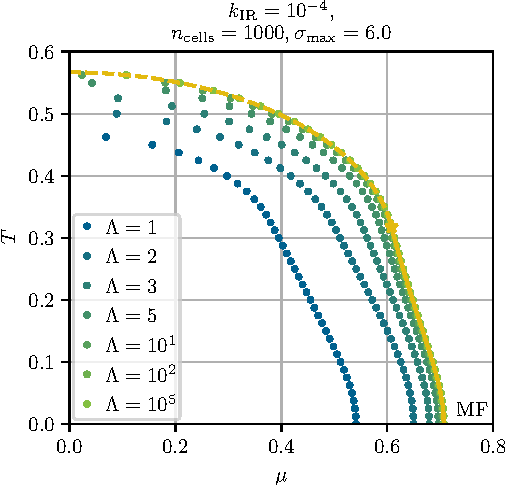
\includegraphics[width=7cm]{gn/figures/MF_consistency_check.pdf}}% Graphics
	[]% Sublabels
	{%
		Phase transition lines (equally colored dots) in the $\mu$-$T$-plane of the \gnym{}~\eqref{eq:bgn-model} in the mean-field approximation for different values of the \uv{} scale $\Lambda$. The curves are extracted from numerical solutions of the \frg{} flows of $u ( t, \sigma )$ with the methods presented in \cref{paragraph:chemical_potential_shock_wave}. As a reference curve, we also plot the exact phase transition line (in yellow) in the renormalized limit $\Lambda\rightarrow\infty$ below the data points, \cf{}\ \cref{fig:GNlargeN_PD}. \Frg{} flows for larger cutoffs $\Lambda$ are closer to the renormalized reference result.
		\fromFig{3}{Stoll:2021ori}
	}%Caption
	{fig:MF_consistency_check}%Label
This paragraph is dedicated to a consistency check of our numeric implementation of the fermionic contribution to the \frg{} flow.
Furthermore, we comment on the concept of \rgcy{} in the context of the discussed mean-field calculations, as a direct application of the first scenario described in \cref{subsubsec:rgcICS}.\bigskip
	
For the consistency checks in this section we use the numerical implementation presented in \cref{paragraph:chemical_potential_shock_wave} and manually switch off the bosonic contribution (the diffusion) in the flow equation \eqref{eq:pdeq-u}.
Since \cref{eq:pdeq-u} is formulated for $u ( t, \sigma ) = \partial_\sigma  U ( t, \sigma )$, we used the $\sigma$-derivative of \cref{eq:initial-condition} as the \ic{} for $u ( t, \sigma )$. Furthermore, as already done in the previous \cref{sec:gnInfHomo}, we work in rescaled quantities. 
This means that $\sigma$ is measured in multiples of $\sigma_0$ and dimensionful quantities are measured in multiples of the Yukawa coupling $h$ \dash{} implying \wlogA{} $h = 1$ and $\sigma_0 = 1$ on the level of the equations. Thus, the \uv{} \ic{} for the (numeric) \frg{} flow in dimensionless variables explicitly reads
\begin{align}
	 u ( t = 0, \sigma ) = \, & \tfrac{d_\gamma}{2 \piu} \, \sigma \, \bigg[ \mathrm{artanh} \bigg( \Big[ 1 + \big( \tfrac{1}{\Lambda} \big)^2 \Big]^{- \frac{1}{2}} \bigg) - \Big[ 1 + \big( \tfrac{1}{\Lambda} \big)^2 \Big]^{- \frac{1}{2}} \bigg] \, .	\label{eq:initial-condition_small_u}
\end{align}
The explicit dependence on $\Lambda$ of $u ( t = 0, \sigma )$ realizes non-trivial \ir{} minima at $\pm\sigma_0$ independent of the \uv{} initial scale by a \rgct{} construction in vacuum.

One way to ensure \rgcy{} in medium is to choose $\Lambda$ significantly larger than all external scales of the problem under consideration.
We will discuss this on mean-field level in this subsection while dedicating \cref{subsec:gnyFiniteNresults} to a similar discussion at finite $N$.\bigskip
	
While the condensate is fixed in the \ir{} in vacuum by construction, the corresponding sigma curvature mass, see \cref{eq:msigma_MF_Lambda}, is not.
Comparing the expression \eqref{eq:msigma_MF_Lambda} at finite $\Lambda$ to the renormalized result of \cref{eq:msigma_MF} we conclude that a relative difference of for example $10^{-3}$ ($10^{-6}$) between $m_\sigma^2$ at finite and infinite $\Lambda$ requires an \uv{} initial scale of around $40$ ($1200$).
Considerations like this in vacuum give insight into internal model scales.
	
Studying the $\Lambda$-dependence of observables at $\mu>0$ and/or $T>0$ we can asses the relation between $\Lambda$ and the external model scales.
To this end we plot the phase transition lines in the $\mu$-$T$-plane, which we obtain via the numerical solution of the purely fermionic \frg{} flow equation for various $\Lambda$ in \cref{fig:MF_consistency_check}. The phase boundaries are extracted via the bisection method~\cite{PresTeukVettFlan92,Press:1992zz} in the $\mu$-$T$-plane, by extracting the minimum of the \ir{} potential from the cell averages $\{ \bar{u}_i ( t_\mathrm{IR} ) \}$.

As reference values for the mean-field phase boundaries in \cref{fig:MF_consistency_check}, we use the exact results of the previous section, which are also plotted in \cref{fig:GNlargeN_PD}. We observe a dependence of the phase boundary between the restored and broken phase on $\Lambda$. Increasing $\Lambda$ beyond $10^2$ we observe an apparent convergence of the numerically obtained phase boundaries, which eventually for $\Lambda \approx 10^5$ approaches the phase boundary of the renormalized mean-field computation. The general \uv{} initial scale dependence at non-zero chemical potential and temperature is easily understood when considering the expression \eqref{eq:rg-U-MF} of the underlying \ir{} potential. 
In \frg{} based mean-field computations with the Litim regulator the \uv{} initial scale acts basically like a sharp momentum cutoff (with an additional surface term, see also \cref{app:GNlpa}).
	
We find that our numeric implementation of the source term in the \frg{} flow equation \eqref{eq:pdeq-u} is capable of reproducing the conventional mean-field results. Furthermore, we already obtain some estimate for decent \uv{}-cutoffs $\Lambda$ for computations involving bosonic quantum fluctuations.
At this point we can close all our preliminary discussions and finally turn our attention to bosonic quantum fluctuations at finite $N$.

\subsection{Bosonic quantum fluctuations in the GNY model}
\label{subsec:gnyFiniteNresults}
\begin{disclaimer}
	In this subsection we closely follow the discussion of results presented in Sec. VI of \nbccite{Stoll:2021ori}.
\end{disclaimer}
In this subsection, we present our (numeric) results for \frg{} flows of the \gnym{} at non-zero $\mu$ and $T$ including bosonic quantum fluctuations in the \lpa.
Thereby we proceed as follows: First, we discuss the dynamics, which take place during a single \frg{} flow at some fixed finite $N$, $\mu$, and $T$, \cf{} the similar discussion in \cref{paragraph:ONadvDif} for the zero-dimensional $O(N)$ model.
This sets the stage for a detailed discussion of the effects that are induced by the chemical potential at low temperatures.
Here we support our conceptual discussion of \cref{paragraph:chemical_potential_shock_wave} with explicit numerical computations.
Afterward, we turn to our central result \dash{} the absence of spontaneous \ZII{} symmetry breaking at finite $N$ and $T > 0$.
We thereby present details on dependencies on $\mu$, $T$, and $N$ of the restoration scale $k_\mathrm{res}$, where the discrete chiral symmetry is restored, as well as a phase diagram during the \frg{} flow.

\subsubsection{Symmetry breaking and restoration during the FRG flow}
\subcaptionFigureVariableWidth%
	[t]% placement
	[0cm]% widthShift
	{% figA
		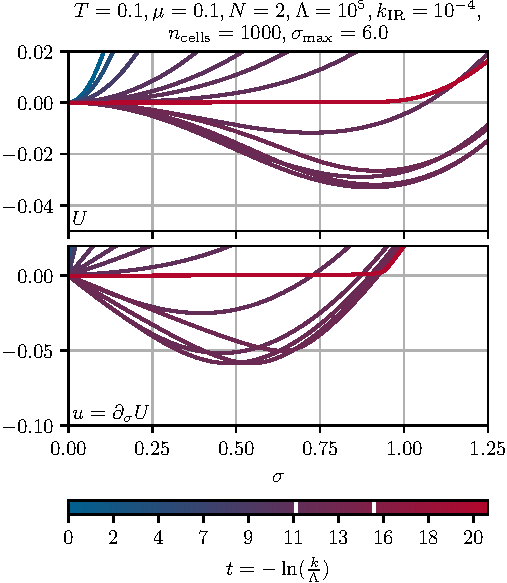
\includegraphics[width=\subcaptionFigureWidth]{gn/figures/flow_N=2,T=0.1,mu=0.1.pdf}% figure (a)
		\captionsetup{font=footnotesize,width=\subcaptionFigureWidth}%
		\caption{
		\frg{} flow of the scale-dependent effective potential $U ( t, \sigma )$ (upper panel) and its $\sigma$-derivative (the fluid) $u ( t, \sigma ) = \partial_\sigma U ( t, \sigma )$ (lower panel) from the \uv{} ({blue}) to the \ir{} ({red}). For the sake of simplicity (and using the (anti-)symmetry in $\sigma$) the functions $u ( t, \sigma )$ and $U ( t, \sigma )$ are plotted for positive $\sigma$ only. The different \rgtimes{} are encoded via the colored bar-legend below the plots. The white vertical lines in the colored bar-legend denote the \rgtimes{} (scales) when the \ZII{} symmetry is broken (condensation) and restored (vaporization).
		}% caption (a)
		\label{fig:flow_N=2T=0.1mu=0.1}% label (a)
	}
	{\hspace{\subcaptionFigureSpacing}}% spacing
	{% figB
		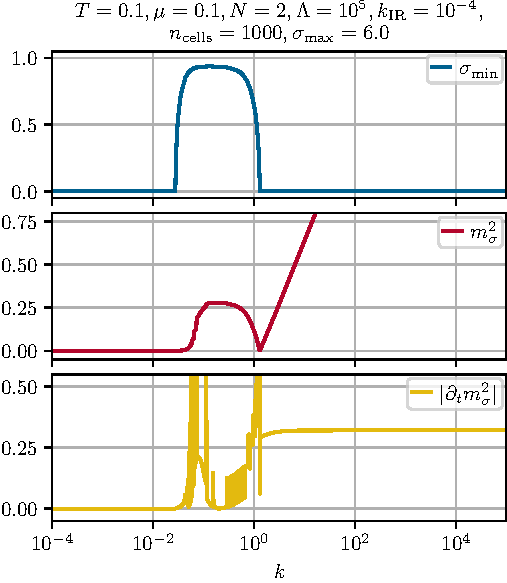
\includegraphics[width=\subcaptionFigureWidth]{gn/figures/k_N=2,T=0.1,mu=0.1.pdf}% Figure (b)
		\captionsetup{font=footnotesize,width=\subcaptionFigureWidth}%
		\caption{%
			\frg{} flow of the minimum $\sigma_{\mathrm{min}} ( k )$ (upper panel), the squared curvature mass $m_\sigma^2 ( k ) = \partial_\sigma u ( t, \sigma )|_{\sigma_\mathrm{min} ( t )}$ at the moving minimum $\sigma_\mathrm{min} (t)$ (middle panel), and the relative change of the squared curvature mass $| \partial_t m_\sigma^2 ( k ) |$ (lower panel) according to \cref{eq:changing_rate_mass} plotted as functions of the \rgscale{} $k ( t )$. Note, that the curvature mass at the moving minimum in the \ir{} is non-zero, $m_\sigma^2 ( t_\mathrm{IR} ) \approx 4.60\cdot10^{-4}$.
		}% caption (b)
		\label{fig:k_N=2T=0.1mu=0.1}% label (b)
	}
	{%
		\frg{} flow of the potential $U(t,\sigma)$ and its derivative on the left \subref{fig:flow_N=2T=0.1mu=0.1} and corresponding evolution of $\sigma_{\mathrm{min}} ( k )$, $m_\sigma^2 ( k )$
		and changing rate $| \partial_t m_\sigma^2 ( k ) |$ on the right \subref{fig:k_N=2T=0.1mu=0.1} for $N=2$ at $T = 0.1$ and $\mu = 0.1$.
		\fromFigs{4 and 5}{Stoll:2021ori}
	}% caption
	{fig:N=2T=0.1mu=0.1}% label
This subsubsection is dedicated to an instructive discussion of symmetry breaking and restoration during \frg{} flows in the framework developed within \cref{sec:0dON}.
To get a better intuition on how this realizes during the \frg{} flow and how the typical setup and dynamics looks like, we picked a single point in the $\mu$-$T$-plane, namely $\mu = 0.1$ and $T = 0.1$, where we at least expect some non-trivial condensation and vaporization phenomena and typical dynamics in the \frg{} flow. We also fixed the number of fermions to $N = 2$.
The computational parameters used for the computations in this subsection are $\sigma_\mathrm{max}=6$, $n_\mathrm{cells}=1000$, $\Lambda=10^{5}$, and $k_\mathrm{IR}=10^{-4}$.
They have been validated with the methodology developed in \cref{subsec:0dONresults} and the detailed checks and numerical tests can be found in \gnAppNum{}.
As \uv{} initial condition, we directly use \cref{eq:initial-condition_small_u}, as discussed in \cref{subsec:UUV}, with $h=1$ and $\sigma_0=1$.

Using this setup, we obtain the numeric results for the \frg{} flow of $u ( t, \sigma )$ and $U ( t, \sigma )$.
The latter is reconstructed from the cell averages $\{ \bar{u}_i ( t ) \}$ by direct Riemann summation, \cf{} \cref{eq:riemann_sum} and the corresponding discussion in \cref{subsubsec:sc1}.
The \frg{} flow of the potential is depicted in \cref{fig:flow_N=2T=0.1mu=0.1} with \cref{fig:k_N=2T=0.1mu=0.1} showing the associated evolution of the scale-dependent minimum $\sigma_\mathrm{min} ( t )$ and the scale-dependent curvature mass,
		\begin{align}
		m^2_{\sigma} ( t ) = \, & \partial_\sigma^2 U ( t, \sigma )\big|_{\sigma_{\min}(t)} =	\, \partial_\sigma u ( t, \sigma )\big|_{\sigma_{\min}(t)} \, ,
	\end{align}
which is evaluated at the moving scale-dependent minimum.
We determine the position of the scale-dependent minimum ${\sigma_\mathrm{min} ( t ) = \Delta \sigma \cdot i_\mathrm{min} ( t )}$, by searching for the position $i_\mathrm{min} ( t )$ of cells next to zero-crossings in the list $\{ u ( t, \sigma_i ) \}$ combined with a check of the list $\{ U ( t, \sigma_i ) \}$ for its smallest entry. 
The curvature mass is calculated at this minimum via a simple right-derivative stencil, hence $\partial_\sigma u ( t, \sigma ) \big|_{\sigma_\mathrm{min} ( t )} = \frac{1}{\Delta \sigma} \, [ \bar{u}_{i_\mathrm{min} + 1} ( t )- \bar{u}_{i_\mathrm{min}} ( t ) ]$.
For optical guidance and better detection, when the plateau in \ir{} is reached, we also introduce the changing rate of the curvature mass
	\begin{align}
		\partial_t m_\sigma^2 ( k_j ) \equiv - k_j \, \frac{m^2_\sigma( k_{j + 1} ) - m^2_\sigma ( k_j )}{  k_{j + 1} - k_j} \, ,	\label{eq:changing_rate_mass}
	\end{align}
which we evaluated for the plots at $j \in \{ 0, 1, \ldots, 998 \}$ intermediate \rgscales{} $k_j$ between $k = \Lambda$ and $k = k_\mathrm{IR}$, such that the belonging \rgtimes{} are equidistantly distributed.

In \cref{fig:N=2T=0.1mu=0.1} we observe the following dynamics: The flow for $u ( t, \sigma )$ starts with the \uv{} initial condition that is linear in $\sigma$. At the beginning of the flow the fermions are active and clearly dominate the dynamics, according to the sink/source contribution in the fluid-dynamic language. We find that this sink/source contribution causes the \ZII{} symmetry breaking and generation of a non-trivial minimum at $k(t \approx  11.2) \approx 1.31$, which is roughly at the order of the model scales, which are of order $1$ (\textit{cf.} position of the intermediate minimum or value of $h$). Shortly after the non-trivial minimum has formed, the sink (source) is still active, but the diffusion caused by the bosonic contributions sets in, due to the negative gradients $\partial_\sigma u ( t, \sigma )$ close to $\sigma = 0$, which enhance the diffusion coefficient. Interestingly, when the position of the minimum (the value of the condensate) has settled, it is approximately of the same order of magnitude as for the mean-field calculations, even though $N = 2$ is everything but close to $N \rightarrow \infty$. As a matter of fact, this signals that the diffusion is weak at $\sigma > \sigma_\mathrm{min} ( t )$. Subsequently, for approximately another two orders of magnitude in \rgscale{} $k ( t )$, the minimum keeps its position $\sigma_\mathrm{min} \approx 0.93$. Also the bosonic curvature mass seems to freeze at $m_\sigma^2 \approx 0.28$ and the potential $U ( t, \sigma )$ is not changing much. However, having a closer look at $u ( t, \sigma )$, we find that the diffusion in field space direction $\sigma$ causes some highly non-linear dynamics, especially close to the point, where the gradient $\partial_\sigma u ( t, \sigma )$ changes its sign. Suddenly, at $k ( t \approx 15.1) \approx 2.76\cdot10^{-2}$, we observe a destabilization of the condensate $\sigma_\mathrm{min} ( t )$ and also $m_\sigma^2 ( t )$ starts changing drastically. The inclusion of \ir{} modes in a small momentum range leads to a complete vaporization of the condensate. Additionally, inspecting $U ( t, \sigma )$, we find that meanwhile the potential turned convex \dash{} as it should be the case in the \ir{}. This flattening of the potential is completely driven by the highly non-linear diffusion, \cf{} \cref{subsec:0dO1Entropy}. Finally, we find that the dynamics completely freezes and that we indeed integrated out all fermionic and bosonic quantum fluctuations. This can be seen best by looking at the absolute value of the changing rate of the squared curvature mass $| \partial_t m_\sigma^2 ( t ) |$, but also directly from $m_\sigma^2 ( t )$ or $\sigma_\mathrm{min} ( t )$. Note, that $m_\sigma^2 ( t_\mathrm{IR} ) \approx 4.60\cdot10^{-4}$, which is not visible from the plot, while $\sigma_\mathrm{min} ( t ) = 0$ already shortly after $k ( t \approx 15.1) \approx 2.76\cdot10^{-2}$.

Overall, we observed that the fermions were indeed able to form a condensate, which however does not survive the long-range bosonic quantum fluctuations in the deep \ir{}. This dynamics might also be referred to as precondensation~\cite{Boettcher:2012cm,Boettcher:2012dh,Boettcher:2013kia,Boettcher:2014tfa,Roscher:2015xha,Khan:2015puu}.

\subsubsection{The role of the chemical potential in the fluid-dynamic setup}\label{subsubsec:chemical_potential_mf_vs_with_bosons}
\fullWidthTwoColumnSubFigures%
	[!t]% Placement
	{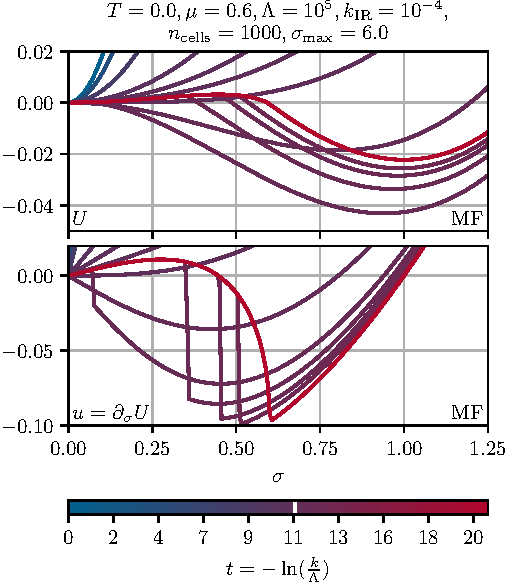
\includegraphics[width=\subcaptionFigureWidth]{gn/figures/flow_MF_T=0.0,mu=0.6.pdf}}% Left figure (dummy index a)
	{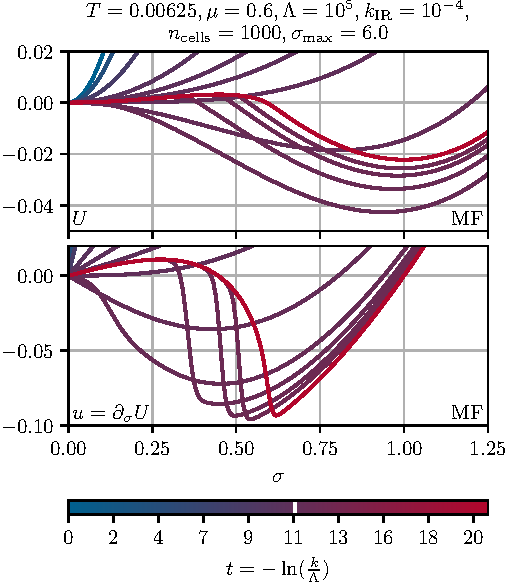
\includegraphics[width=\subcaptionFigureWidth]{gn/figures/flow_MF_T=0.00625,mu=0.6.pdf}}% Right figure (dummy index b)
	[fig:flow_MF_T=0.0mu=0.6,fig:flow_MF_T=0.00625mu=0.6] %Labels
	{%
		Mean-field (infinite-$N$) \frg{} flow (sink term only) of the scale-dependent effective potential $U ( t, \sigma )$ (upper panel) and its $\sigma$-derivative (the fluid) $u ( t, \sigma )$ (lower panel) from the \uv{} ({blue}) to the \ir{} ({red}).
		For $T=0$ on the left~\subref{fig:flow_MF_T=0.0mu=0.6} and $T=0.00625$ on the right~\subref{fig:flow_MF_T=0.00625mu=0.6} both at $\mu=0.6$.
		The white vertical line in the colored bar-legend denotes the \rgtime{} (scales) when the \ZII{} symmetry is broken (condensation).
		There is no symmetry restoration at these points in the phase diagram in \mf{}.
		\fromFigs{6 and 7}{Stoll:2021ori}
	}% Caption
	{fig:flow_MFmu=0.6}% Label
	
Before we come to our discussion on symmetry breaking and restoration in \frg{} flows for arbitrary $N$ and arbitrary points in the $\mu$-$T$-plane, we briefly return to the discussion in \cref{paragraph:chemical_potential_shock_wave} on the role of the chemical potential in the fluid-dynamic formulation of the \frg{} flow equation \eqref{eq:pdeq-u}. We therefore accentuate our theoretical discussion with explicit calculations and plots of \frg{} flows at very low as well as vanishing temperature and moderate chemical potential. \WlogA{} we choose $\mu = 0.6$ and $T = 0.00625$ or $T = 0$.\bigskip

Therefore we present \cref{fig:flow_MF_T=0.0mu=0.6} as the reference plot of our discussion. It shows the mean-field \frg{} flow for $u ( t, \sigma )$ and $U ( t, \sigma )$ at $T = 0$ and $\mu = 0.6$. As predicted the chemical potential enters the \frg{} flow of $u ( t, \sigma )$, which is entirely described via the source/sink equation, suddenly as a discontinuity of $u ( t, \sigma )$ in field space. This discontinuity appears at $\sigma = 0$ when $k^2 ( t ) \approx \mu^2$ and moves towards larger $| \sigma |$ until $\sigma^2 \approx \tfrac{\mu^2}{h^2}$ ($h = 1$). Formally, this discontinuity leads to infinite negative gradients $\partial_\sigma u ( t, \sigma )$ and impedes the following study of bosonic quantum fluctuations at $T = 0$, $\mu \neq 0$ and finite $N$. This is, because $E^2_\mathrm{b} ( t, \partial_\sigma u ) = k^2 ( t ) + \partial_\sigma u ( t, \sigma ) \approx \mu^2 + \partial_\sigma u ( t, \sigma ) < 0$, which leads to an abrupt overshooting over the poles of the bosonic propagators $\tfrac{1}{E_\mathrm{b}}$ and drives the diffusion coefficient $\alpha ( t, \partial_\sigma u )$ from \cref{eq:heat_equation_analogy} negative.

After spatial integration of $u ( t, \sigma )$ the remnant of the discontinuity is clearly visible in $U ( t, \sigma )$ in terms of a moving cusp. Additionally, it is worth mentioning that the potential $U ( t, \sigma )$ is in the symmetry broken phase and everything but flat for small $|\sigma|$ in the \ir{}, which violates a fundamental property of thermodynamic potentials and $\Gamma [ \varphi, \psi,\bar{\psi}]$, namely convexity. This is a typical mean-field/infinite-$N$ artifact.\bigskip

In order to study, how the chemical potential influences the bosonic \frg{} flows, hence the diffusion in field space, we first slightly increase the temperature of the mean-field calculation to $T = 0.00625$, while keeping the same chemical potential $\mu = 0.6$. In \cref{fig:flow_MF_T=0.00625mu=0.6} it is clearly visible that the huge negative gradients $\partial_\sigma u ( t, \sigma )$ are still present and the overall shape and flows of $u ( t, \sigma )$ and $U ( t, \sigma )$ do not change much compared to \cref{fig:flow_MF_T=0.0mu=0.6}.

Though, already very small temperatures are able to smear out the sharp edges of the jumps, which smoothens $u ( t, \sigma )$ significantly already without any diffusive contributions from the bosons. This effect stemming from the Fermi-Dirac distribution function \eqref{eq:nfDef} enables the inclusion of bosons, since gradients are still large, but finite.\bigskip

\fullWidthTwoColumnSubFigures%
	[!t]% Placement
	{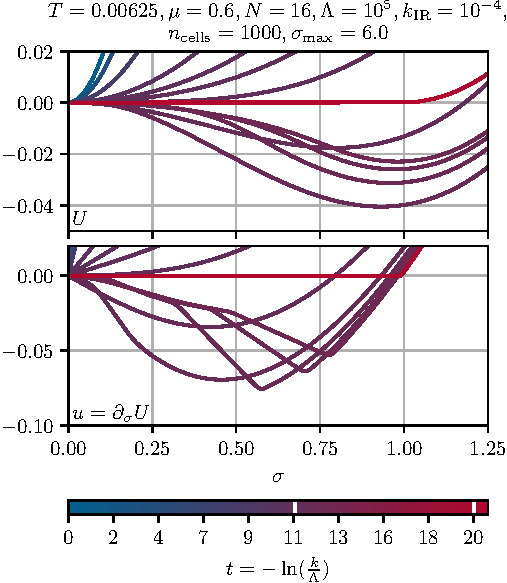
\includegraphics[width=\subcaptionFigureWidth]{gn/figures/flow_N=16,T=0.00625,mu=0.6.pdf}}% Left figure (dummy index a)
	{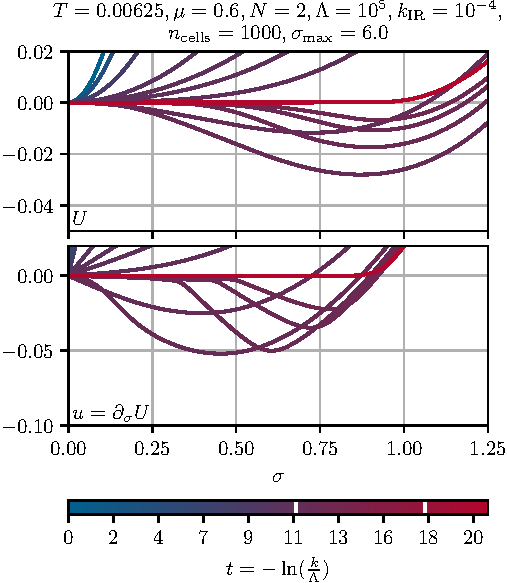
\includegraphics[width=\subcaptionFigureWidth]{gn/figures/flow_N=2,T=0.00625,mu=0.6.pdf}}% Right figure (dummy index b)
	[fig:flow_N=16T=0.00625mu=0.6,fig:flow_N=2T=0.00625mu=0.6] %Labels
	{%
		Same \frg{} flow as in \cref{fig:flow_MF_T=0.00625mu=0.6} but $N = 16$ on the left \subref{fig:flow_N=16T=0.00625mu=0.6}  and $N=2$ on the right \subref{fig:flow_N=2T=0.00625mu=0.6} instead $N\rightarrow\infty$, thus involving the effects of bosonic quantum fluctuations (diffusion).
		\fromFigs{8 and 9}{Stoll:2021ori}
	}% Caption
	{fig:flowmu=0.6}% Label
	
The next question is, what happens, if the number of fermions is finite and bosonic fluctuations enter the \frg{} flow as non-linear diffusion on the level of $u ( t, \sigma )$. To this end, we plot the same \frg{} flows as before at $T = 0.00625$ and $\mu = 0.6$ for $N = 16$ fermions in \cref{fig:flow_N=16T=0.00625mu=0.6}.

Even though the number of fermions seems to be rather large, the overall picture changes drastically when compared to the situation in the limit $N\rightarrow\infty$. We observe that the chemical potential is still clearly visible on the level of $u ( t, \sigma )$ in terms of rather large gradients and cusps. But it is hardly visible in $U ( t, \sigma )$. The highly non-linear character of the diffusion does not really smear out the cusps, but results in the somewhat strange movement of the straight part of $u ( t, \sigma )$ between the two pronounced edges. Finally, the greatest difference to the mean-field calculations is that the diffusion vaporizes the condensate and fully restores the \ZII{} symmetry in the \ir{}\footnote{We have checked numerically that there is indeed only a trivial minimum at $\sigma = 0$, which is hardly visible, because $u ( t_\mathrm{IR}, \sigma )$ and $U ( t_\mathrm{IR}, \sigma )$ are extremely close to the $\sigma$-axis in the relevant region. For details, we refer to the discussions within the next subsubsections.}. Additionally, the potential $U ( t, \sigma )$ turns convex in the \ir{}, as expected in the case of finite $N$. Already from this calculation it is obvious that large but finite numbers of $N$ yields entirely different results than the $N \rightarrow \infty$ limit, as prominently stated in various publications~\cite{Witten:1978qu,ZinnJustin:2002ru,Rosenstein:1990nm} and exemplified in great detail in \cref{subsec:0dLargeN} for the zero-dimensional $O(N)$ model at large $N$.\bigskip

\fullWidthTwoColumnFigures%
	[!t] % Placement
		{%
		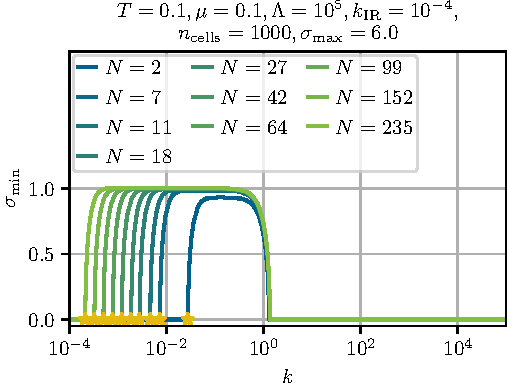
\includegraphics[width=\subcaptionFigureWidth]{gn/figures/Nf_k_sigma_min.pdf} % left figure
		\captionsetup{width=\subcaptionFigureWidth}%
		\caption{%
			\frg{} flows of the value of the condensate (the position of the minimum) $\sigma_{\mathrm{min}} ( k )$ for various $N$ as functions of the \rgscale{} $k$ at $T = 0.1$ and $\mu = 0.1$. The yellow stars mark the \rgscales{} $k_\mathrm{res}$, where the \ZII{} symmetry is restored, signaled by a vanishing condensate.
			\fromFig{10}{Stoll:2021ori}
		}
		\label{fig:Nf_k_sigma_min}
	}
	{\fullWidthTwoColumnFigureSpacing}
	{%
		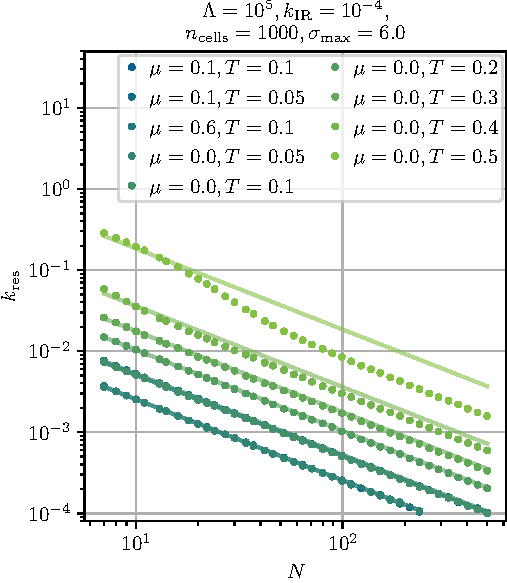
\includegraphics[width=\subcaptionFigureWidth]{gn/figures/Nf_k_restored.pdf} % Right figure
		\captionsetup{width=\subcaptionFigureWidth}%
		\caption{%
			Restoration scale $k_\mathrm{res}$, where the \ZII{} symmetry is restored during the \frg{} flow, as a function of the number of fermions $N$ at various points in the $\mu$-$T$-plane, where the \ZII{} symmetry was dynamically broken at $k > k_\mathrm{res}$ by the fermions. For $\mu = 0.1$ and $T = 0.1$ the data points correspond to the yellow stars in \cref{fig:Nf_k_sigma_min}. For the various ($\mu$,$T$)-tuples we include $k_\mathrm{res} ( N ) \propto N^{-1}$ fits ought to be used for optical guidance. Note, that the points for equal temperatures but different chemical potentials are lying on top of each other. In \cref{subsubsec:variablemu} we will discuss this in detail.
			\fromFig{11}{Stoll:2021ori}%
		}%
		\label{fig:Nf_k_restored}
	}%
\FloatBarrier
Finally, we further decrease the number of fermions to $N = 2$ and again study the \frg{} flows at $T = 0.00625$ and $\mu = 0.6$. In the corresponding \cref{fig:flow_N=2T=0.00625mu=0.6} we observe that the diffusion via the \sigmaMode{} sets in much earlier during the \frg{} flow and the intermediate symmetry breaking is less drastic. The reason is rather obvious: Changing $N$ in \cref{eq:zero_t_flow_equation} changes the relative strength between bosonic and fermionic interactions (fluctuations). On the level of the fluid-dynamic equation \eqref{eq:pdeq-u} this implies that the flow is either more diffusion (for small $N$) or more source/sink (for large $N$) dominated. Still, even for $N = 2$ the chemical potential is clearly visible in form of a slightly smeared and moving cusp in $u ( t, \sigma )$. Apart from this, the qualitative picture is similar to the $N = 16$ scenario.\FloatBarrier

\subsubsection{Varying the number of flavors \texorpdfstring{$N$}{N}}\label{subsubsec:variableN}
Next, we turn to a more systematic analysis of our previous findings regarding \frg{} flows at different numbers of flavors. We start by analyzing the relation between the \rgscale{} $k_\mathrm{res}$, where the \ZII{} symmetry is restored (if it was initially broken by fermionic quantum fluctuation) and the number of fermionic flavors $N$.\bigskip
	
As a first step to get an overall impression, we again fix $\mu = 0.1$ and $T = 0.1$ and look at the condensate $\sigma_\mathrm{min} ( t )$ as a function of the \rgscale{} $k ( t )$ for various selected values of $N$. The numeric results are depicted in \cref{fig:Nf_k_sigma_min}.

The results are rather intuitive. The \rgtime{} period, in which we find a non-zero condensate ${\sigma_\mathrm{min} ( t ) \neq 0}$, strongly depends on $N$. For small $N$, the \ZII{} symmetry restores almost at model scales, which are set by $h = 1$, while for larger $N$ one finds that the restoration scale $k_\mathrm{res}$ moves several orders of magnitude on the \rgscale{} towards the \ir{}\footnote{This is the reason, why we cannot choose arbitrarily large $N$ for numeric calculations. If $N$ is too large, we have to integrate to too small \rgscales{} to find symmetry restoration. However, this is numerically not possible, due to general limitations of the numerical precision during numerical \rgtime{} evolution.}. Furthermore, we observe that in the time periods with broken \ZII{} symmetry, the position of the minimum $\sigma_\mathrm{min} ( t )$ is approaching its mean-field value ${\sigma_\mathrm{min} = 1}$ rapidly while increasing $N$ in \cref{fig:Nf_k_sigma_min}. The reason for this behavior is that the precondensation \dash{} the formation of a non-persistent non-trivial minimum during the \frg{} flow \dash{} due to fermionic quantum fluctuations does not depend on $N$.\bigskip

The direct follow up question is, if there is some fixed relation between $k_\mathrm{res}$ and $N$ and if we can expect to recover the mean-field result for $N \rightarrow \infty$, where $k_\mathrm{res} = 0$, which is not reachable in practical computations at finite $N$ involving bosonic fluctuations. Therefore, we calculate and plot $k_\mathrm{res}$ as a function of $N$ for different combinations of $\mu$ and $T$ in \cref{fig:Nf_k_restored} in a double logarithmic plot. The values for $\mu$ and $T$ in \cref{fig:Nf_k_restored} lie in the symmetry broken phase of the MF phase diagram and consequently precondensation occurs during the \frg{} flow, which is necessary to define and discuss the restoration scale $k_\mathrm{res}$.

Already from the numeric data points, it seemed as if we found some power law behavior for $k_\mathrm{res} ( N )$, which was confirmed for all combinations of $\mu$ and $T$, as long as $T$ is sufficiently small\footnote{For $\mu = 0.0$ and $T = 0.5$ the relation $k_\mathrm{res} ( N )$ does not obey a strict power law \eqref{eq:N-k} but slightly deviates. We believe that the reason for this behavior is the fact that for sufficiently large $T$ one is already close to the second-order phase transition, where the \ZII{} symmetry is restored by thermal fluctuations (also in mean-field) and not primary by bosonic quantum fluctuations.}. The straight lines are fits of the function
	\begin{align}
		k_{\mathrm{res}} ( N ) \propto N^{-1}	\label{eq:N-k}
	\end{align}
to our data points. This strongly supports the hypothesis that for all finite $N$ the discrete chiral symmetry is never broken in the \ir{} for $T>0$, while for $N \rightarrow \infty$, the mean-field result is recovered. In the following discussions we will mainly focus on $N = 2$. Nevertheless, we checked for various other values of $N$ that our overall findings are similar for general finite $N > 1$.

\subsubsection{Varying the temperature \texorpdfstring{$T$}{T}}\label{subsubsec:variableT}
\fullWidthTwoColumnFigures%
	[!t] % Placement
	{%
		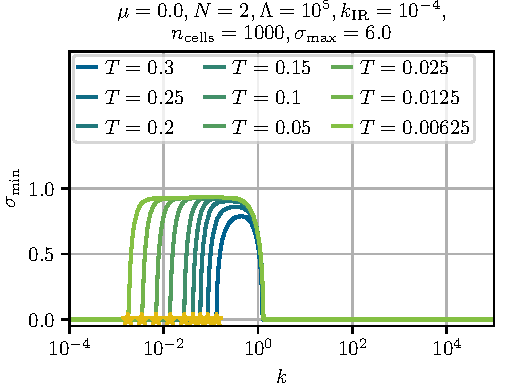
\includegraphics[width=\subcaptionFigureWidth]{gn/figures/T_k_sigma_min.pdf} % left figure
		\captionsetup{width=\subcaptionFigureWidth}%
		\caption{%
			Value of the condensate (the position of the minimum) $\sigma_{\mathrm{min}} ( k )$ for various $T$ as a function of the \rgscale{} $k ( t )$. The yellow stars mark the \rgscales{} $k_\mathrm{res}$, where the \ZII{} symmetry is restored, signaled by a vanishing condensate.
			\fromFig{12}{Stoll:2021ori}
		}
		\label{fig:T_k_sigma_min}
	}
	{\fullWidthTwoColumnFigureSpacing}
	{%
		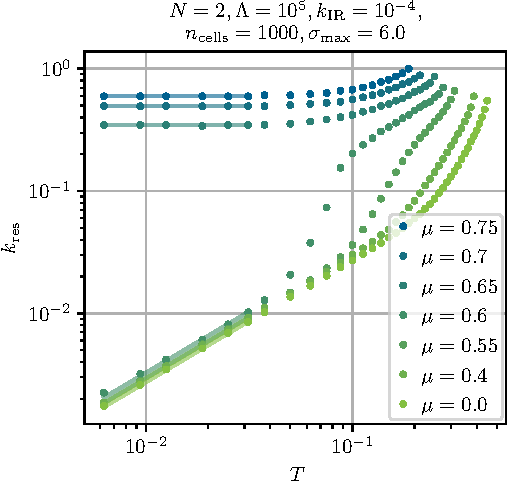
\includegraphics[width=\subcaptionFigureWidth]{gn/figures/T_k_restored.pdf} % Right figure
		\captionsetup{width=\subcaptionFigureWidth}%
		\caption{%
			Restoration scale $k_\mathrm{res}$, where the \ZII{} symmetry is restored during the \frg{} flow, as a function of temperature $T$ for a constant number of fermionic flavors $N = 2$ and various values of $\mu$. The points corresponding to ${\mu = 0.65}$, ${\mu = 0.7}$, and ${\mu = 0.75}$ correspond to regions in the $\mu$-$T$-plane, where the \ZII{} symmetry is restored by the chemical potential, already before bosonic fluctuations are active, \cf{} \cref{fig:phase_boundaries}. For temperatures larger than the points, which are shown in the plot, there is never symmetry breaking throughout the entire \frg{} flow. For $T\smallerlesssim 0.03$ we plot $k_{\mathrm{res}}(T) \propto T^{0}$ for $\mu>0.6$ and $k_{\mathrm{res}}(T) \propto T$ for $\mu<0.6$ ought to be used for optical guidance.
			\fromFig{13}{Stoll:2021ori}%
		}%
		\label{fig:T_k_restored}
	}%

	In this subsubsection we focus on the relation between the restoration scale $k_\mathrm{res}$ and the temperature $T$. This relation is exemplified for $N = 2$.\\
	
	We start by setting $\mu = 0$ and solely focusing on the evolution of $\sigma_\mathrm{min} ( t )$ along the \rgscale{} $k ( t )$ for different temperatures $T$. This is plotted in \cref{fig:T_k_sigma_min}.

		
	We find, that by decreasing the temperature, the \rgtime{} period of broken \ZII{} symmetry becomes longer and one has to go deeper into the \ir{} to find symmetry restoration for smaller temperatures. Additionally, we observe remnants of the mean-field second-order phase transition, because for larger temperatures the value of the intermediate condensate $\sigma_\mathrm{min} ( t )$ is smaller than for smaller temperatures. In general we observe no \ssb{} in the \ir{} for all $T>0$ and $\mu=0$. For temperatures above the mean-field critical temperature $T_\mathrm{C}\simeq  0.567$, see \cref{eq:Tc_MF}, symmetry restoration is driven by thermal fluctuations while for $0 < T < T_\mathrm{C}$ bosonic quantum fluctuations seem to drive symmetry restoration at finite $N$ and $\mu = 0$.\\	

	In \cref{fig:T_k_restored} we present results for the temperature-dependence of the symmetry restoration scale $k_\mathrm{res} ( T )$ for various chemical potentials.  We observe that for large temperatures, which are already close to the mean-field critical temperature, the influence of the thermal fluctuations, also in the fermionic loop contribution is too large to have a simple relation between $k_\mathrm{res}$ and $T$. For $T\smallergtrsim 0.03$ we find that $k_\mathrm{res} ( T )$ depends non-trivially on $\mu$ indicating a complicated interplay of thermal, density, and quantum fluctuations that leads to symmetry restoration.
	
	For low temperatures we can identify two distinct trends in \cref{fig:T_k_restored}. On the one hand, the points $k_\mathrm{res} ( T )$ for $\mu>0.6$ become insensitive to $T$ for $T \smallerlesssim 0.03$ while showing a clear dependence on $\mu$: $k_\mathrm{res} ( T ) = c ( \mu ) \, T^0$. In this regime it is not the bosonic quantum fluctuations that restore the symmetry, but rather density fluctuations related to the chemical potential. This is already the case in the limit $N \rightarrow \infty$ (mean-field). In the fluid-dynamical interpretation of fermions as a source/sink term, symmetry gets restored at large chemical potentials due to the manifestation as a source in this scenario, \cf{} \cref{paragraph:chemical_potential_shock_wave}.
	
	On the other hand, the points $k_\mathrm{res} ( T )$ for $\mu < 0.6$ become rather insensitive to $\mu$ for $T \smallerlesssim 0.03$ while showing a clear linear dependence on $T$, \textit{viz.} $k_\mathrm{res} ( T ) = c ( \mu ) \, T$, where the constant $c(\mu)$ depends only very weakly on $\mu$. This implies that for small $T$ the fermionic contributions to the flow are almost negligible and predominantly the first non-zero Matsubara mode $2 \piu  T$ controls $k_\mathrm{res}$, which also explains the linear relation between $k_\mathrm{res}$ and $T$.
	
	For $T<0.3$ and $\mu<0.6$ we find symmetry restoration at a finite $k_\mathrm{res}$ \dash{} consequently no \ssb{} in the \ir{} \dash{} at finite $N = 2$, which is in direct contrast to the $N \rightarrow \infty$ (mean-field) results, where symmetry is still broken in this regime. Assuming that the functional trends identified in \cref{fig:T_k_restored} at low $T$ hold in the limit $T \rightarrow 0$, the linear relations $k_\mathrm{res} ( T ) \propto T^1$ suggest \ssb{} in the \ir{} at $T = 0$ even at finite $N$. We will come back to this possibility in \cref{subsubsec:PDfiniteN} when discussing the phase diagram after we explore the situation in vacuum in \cref{subsubsec:vacFiniteN_LD1}.\\

	Before we turn to further discussion concerning the chemical potential, we conclude this subsubsection on temperature-dependencies with another plot, namely \cref{fig:precondensation_T}. With this figure we study the dependence of the temperature $T_\mathrm{pc}$ on $N$. $T_\mathrm{pc}$ is the precondensation temperature~\cite{Boettcher:2012cm,Boettcher:2012dh,Boettcher:2013kia,Boettcher:2014tfa,Roscher:2015xha,Khan:2015puu}, which is defined in our work as the threshold temperature above which the system is always in the symmetric phase for all $k(t)$ at $\mu = 0$ and \ZII{} symmetry is never broken during the \frg{} flow. We observe that 
	$T_\mathrm{pc}$ approaches the mean-field value for the critical temperature $T_\mathrm{C} \simeq 0.567$ while increasing $N$. It should however be stressed, that for finite $N$ $T_\mathrm{pc}$ is not a critical temperature associated with a second-order phase transition to a symmetry broken phase in the \ir{}. While symmetry breaking occurs for $T < T_\mathrm{pc} ( N )$ during the \frg{} flow, bosonic fluctuations restore symmetry in the \ir{} for all finite $N$. Only in the limit $N \rightarrow \infty$ the mean-field result of a second-order phase transition at $\lim_{N \rightarrow \infty} T_\mathrm{pc} ( N ) = T_\mathrm{C}$ is recovered, which again qualitatively confirms the consistency of our numeric results.\clearpage

\halfWidthFigure%
	{gn/figures/precondensation_T.pdf}
	[]
	{%
		Precondensation temperature $T_\mathrm{pc} ( N )$ as a function of the number of fermions $N$ at $\mu = 0$. Hereby $T_\mathrm{pc} ( N )$ is defined as the temperature that is needed to keep the system in the \ZII{}-symmetric phase over the entire \frg{} flow, meaning that $\sigma_\mathrm{min} ( k ) = 0$ at all scales $k$. The {red-dashed} line marks the critical temperature $T_\mathrm{C}\simeq 0.567$ from mean-field calculations, see \cref{eq:Tc_MF}.
		\fromFig{14}{Stoll:2021ori}
	}%
	{fig:precondensation_T}

\subsubsection{Varying the chemical potential \texorpdfstring{$\mu$}{mu}}\label{subsubsec:variablemu}
To further study the relation between $k_\mathrm{res}$ and $\mu$, we proceed as follows. First, we fix $N = 2$ and $T = 0.1$ and again look at $\sigma_\mathrm{min} ( t )$ plotted over the \rgscale{} $k ( t )$ in \cref{fig:mu_k_sigma_min}.

Here, we observe that for large $\mu>0.6$ the fermionic density fluctuations restore the symmetry during the \frg{} flow, signaled by a $k_\mathrm{res}$ which is slightly smaller than $\mu$ but of the same order of magnitude. The strip at $T=0.1$ with $\mu>0.6$ is in the restored phase of the mean-field phase diagram and the dynamics at finite and infinite $N$ are dominated by fermionic density fluctuations mediated by the chemical potential. Small values of $\mu<0.6$ cannot influence a large region in field space. The source contributions at small $\mu$ are insufficient to restore the symmetry (compare with our previous discussions). For $\mu<0.6$ the restoration scale $k_\mathrm{res}$ is always the same and is set by the temperature.

This behavior is visualized even better in \cref{fig:mu_k_restored}, where we plot $k_\mathrm{res} ( \mu )$ for various $T$.
Note that $k_\mathrm{res} ( \mu )$ becomes insensitive to $\mu$ for small chemical potentials. We observe remnants \dash{} the jump/large gradient in $k_\mathrm{res} ( \mu )$ at $\mu\approx 0.6$ around $T\approx0.3$ \dash{}  of the mean-field first-order phase transition below the mean-field critical point $(\mu_\mathrm{CP},T_\mathrm{CP})\simeq(0.6,0.3)$.\clearpage

\fullWidthTwoColumnFigures%
	[!t] % Placement
	{%
		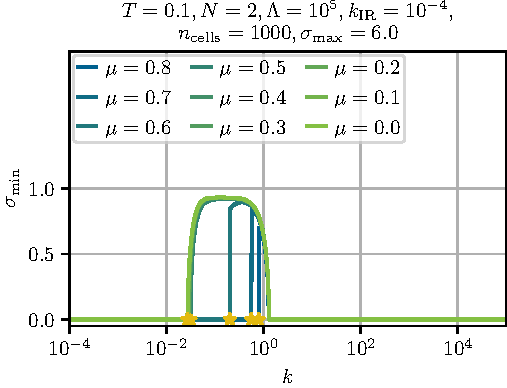
\includegraphics[width=\subcaptionFigureWidth]{gn/figures/mu_k_sigma_min.pdf} % left figure
		\captionsetup{width=\subcaptionFigureWidth}%
		\caption{%
			Value of the condensate (position of the minimum) $\sigma_\mathrm{min} ( k )$ for various $\mu$ as a function of the \rgscale{} $k ( t )$ at constant temperature $T = 0.1$ and constant $N = 2$. The yellow stars mark the \rgscales{}, where the \ZII{} symmetry is restored, signaled by a vanishing condensate.
			\fromFig{15}{Stoll:2021ori}
		}
		\label{fig:mu_k_sigma_min}
	}
	{\fullWidthTwoColumnFigureSpacing}
	{%
		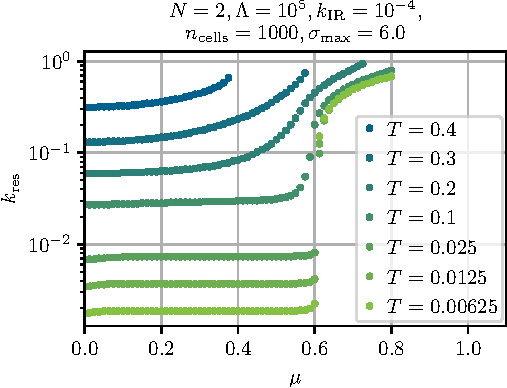
\includegraphics[width=\subcaptionFigureWidth]{gn/figures/mu_k_restored.pdf} % Right figure
		\captionsetup{width=\subcaptionFigureWidth}%
		\caption{%
			Restoration scale $k_\mathrm{res}$, where the \ZII{} symmetry gets restored during the \frg{} flow, as a function of the chemical potential $\mu$ for different temperatures for constant $N = 2$.
			\fromFig{16}{Stoll:2021ori}%
		}%
		\label{fig:mu_k_restored}
	}%
\subsubsection{Computations in vacuum}\label{subsubsec:vacFiniteN_LD1}
\subcaptionFigureVariableWidth%
	[t]% placement
	[0cm]% widthShift
	{% figA
		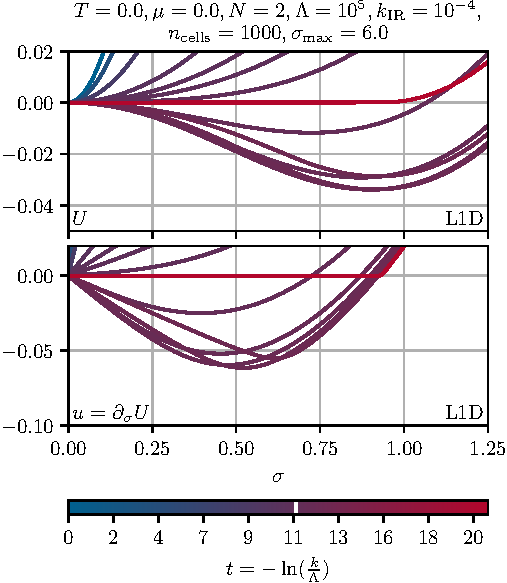
\includegraphics[width=\subcaptionFigureWidth]{gn/figures/flow_L1D_N=2,T=0.0,mu=0.0.pdf}% figure (a)
		\captionsetup{font=footnotesize,width=\subcaptionFigureWidth}%
		\caption{
		\frg{} flow of the scale-dependent effective potential $U ( t, \sigma )$ (upper panel) and its $\sigma$-derivative (the fluid) $u ( t, \sigma )$ (lower panel). The white vertical line in the colored bar-legend denotes the \rgtime{} (scales) when the \ZII{} symmetry is broken (condensation). We do not find symmetry restoration in vacuum for finite $N=2$ within the \frg{} flow for $k\geq k_\mathrm{IR}=10^{-4}$.
		}% caption (a)
		\label{fig:flow_L1D_N2T0mu0}% label (a)
	}
	{\hspace{\subcaptionFigureSpacing}}% spacing
	{% figB
		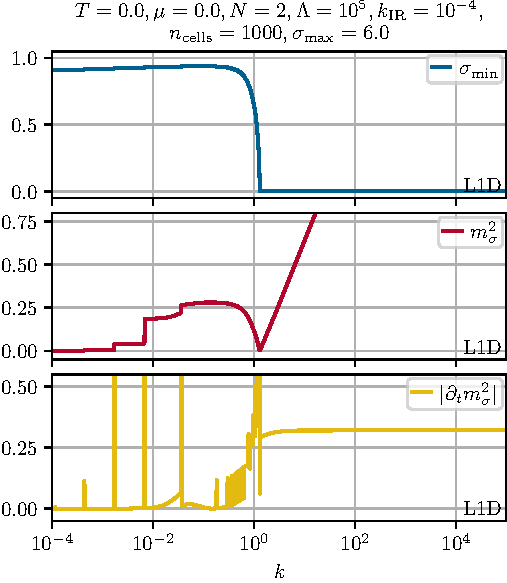
\includegraphics[width=\subcaptionFigureWidth]{gn/figures/k_L1D_N=2,T=0.0,mu=0.0.pdf}% figure (b)
		\captionsetup{font=footnotesize,width=\subcaptionFigureWidth}%
		\caption{%
			\frg{} flow of the minimum $\sigma_{\mathrm{min}} ( k )$ (upper panel), the squared curvature mass $m_\sigma^2 ( k ) = \partial_\sigma u ( t, \sigma )$ (middle panel), and the relative change of the squared curvature mass $| \partial_t m_\sigma^2 ( k ) |$ (lower panel) according to \cref{eq:changing_rate_mass} plotted as functions of the \rgscale{} $k ( t )$ in vacuum ($T = \mu =0$).
		}% caption (b)
		\label{fig:k_L1D_N2T=0mu0}% label (b)
	}
	{%
		\frg{} flow of the potential $U(t,\sigma)$ and its derivative on the left \subref{fig:flow_L1D_N2T0mu0} and corresponding evolution of $\sigma_{\mathrm{min}} ( k )$, $m_\sigma^2 ( k )$
		and changing rate $| \partial_t m_\sigma^2 ( k ) |$ on the right \subref{fig:k_L1D_N2T=0mu0} for $N=2$ in vacuum.
		Results were obtained using the conventional one-dimensional, spatial \lpa{}-optimized (Litim) regulator.
		Corresponding results with the two-dimensional \lpa{}-optimized (Litim) regulator can be found in \gnAppVacFlow{}.
		\fromFigs{17 and 18}{Stoll:2021ori}
	}% caption
	{fig:L1D_N=2,T=0.0,mu=0.0}% label

	Before we conclude this subsection with the discussion of the phase diagram at finite $N$ we turn to selected results in vacuum at vanishing temperature and chemical potential. Direct numerical computations at $T=0$ and $\mu>0$ and finite $N$ were not possible within this work as discussed at length in the previous subsubsections. Computations at $T=0$ and vanishing chemical potential $\mu=0$ are however possible at finite $N$. In this subsubsection we discuss a specific vacuum flow at $N=2$ obtained by numerical solution of the vacuum flow \cref{eq:vacuum_limit_flow_equation} (strictly speaking the $\sigma$-derivative of \cref{eq:vacuum_limit_flow_equation}) with the one-dimensional Litim regulator also used for the previous computations at $T>0$.\\

	The vacuum \frg{} flow for $N=2$ is displayed in \cref{fig:flow_L1D_N2T0mu0}, showing the scale evolution from the \uv{} and the initial condition~\eqref{eq:initial-condition_small_u} towards the \ir{}. The corresponding flows of the running minimum $\sigma_{\mathrm{min}} ( k )$, the squared curvature mass $m_\sigma^2 ( k ) = \partial_\sigma u ( t, \sigma )$ at the \ir{} minimum $\sigma_\mathrm{min}>0$ with the corresponding changing rate  $| \partial_t m_\sigma^2 ( k ) |$ according to \cref{eq:changing_rate_mass} are plotted in \cref{fig:k_L1D_N2T=0mu0}. We observe \ssb{} in the \ir{} indicated by the non-zero minimum $\sigma_\mathrm{min} > 0$. The value of $\sigma_\mathrm{min}\approx 0.907$ for $N = 2$ is slightly smaller than the mean-field value in the limit $N \rightarrow \infty$ of $\sigma_\mathrm{min} = \sigma_0 = 1$. The curvature mass squared for $N = 2$ is extremely small with {$m_\sigma^2 \approx 1.04 \cdot 10^{-5}$,} significantly smaller than the mean-field value of $m_\sigma^2 =\tfrac{1}{\piu}\simeq 0.318$, see \cref{eq:msigma_MF}, in the limit $N \rightarrow \infty$. The changing rate  $| \partial_t m_\sigma^2 ( k ) |$ indicates an extremely long dynamical range in \rgscale{} $k$. The \ir{} cutoff of $k_\mathrm{IR}=10^{-4}$ is arguably not low enough and integration deeper into the \ir{} should be performed to ensure that all relevant long-range bosonic vacuum fluctuations are included. However the computations in vacuum are numerically extremely demanding. Lower \ir{} cutoffs would require better spatial resolution and potentially even higher numerical precession for numerical \rgtime{} evolution. Both increase the computational time significantly. Computations with lower \ir{} cutoffs were infeasible within the scope of this work. This limitation also implicitly excludes studies at significantly higher finite $N$ since the dynamics get shifted to even lower \rgscales{} for $N>2$ as discussed in \cref{subsubsec:variableN}.

	The result of \ssb{} in the \ir{} for finite $N=2$ at $T=\mu=0$ is supported by the results discussed in \gnAppVacFlow{} obtained from vacuum flows using two-dimensional Litim regulators. A non-vanishing $\sigma_\mathrm{min}$ in vacuum is also supported by the results at finite but low temperature of \cref{subsubsec:variableT} and especially the results presented in \cref{fig:T_k_restored}.\clearpage

\subsubsection{The phase diagram}\label{subsubsec:PDfiniteN}
\subcaptionFigureVariableWidthNonAligned%
	[t]% placement
	[0cm]% widthShift
	[\vspace{0.3cm}]% heightShiftLeft
	[\vspace{0cm}]% heightShiftRight
	{%
		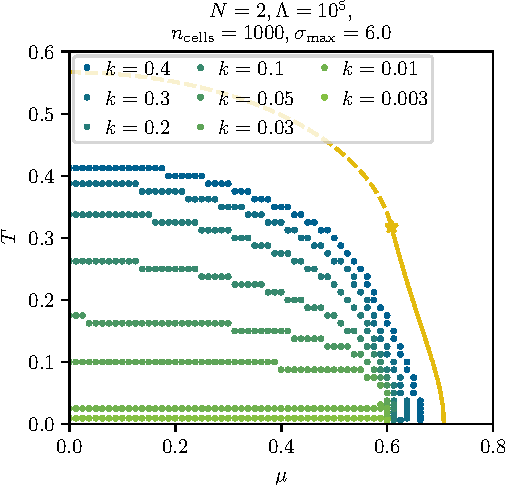
\includegraphics[width=\subcaptionFigureWidth]{gn/figures/phase_boundaries.pdf}% Figure (b)
		\captionsetup{font=footnotesize,width=\subcaptionFigureWidth}%
		\caption{%
				Phase transition lines (equally colored dots) depending on the \rgscale{} $k ( t )$. The yellow solid/dashed line is the mean-field result for the phase transition line and taken from \cref{fig:GNlargeN_PD}. It is only plotted as reference and serves as optical guidance.
		}% Caption (b)
		\label{fig:phase_boundaries}% label (b)
	}
	{\hspace{\subcaptionFigureSpacing}}% spacing
	{%
		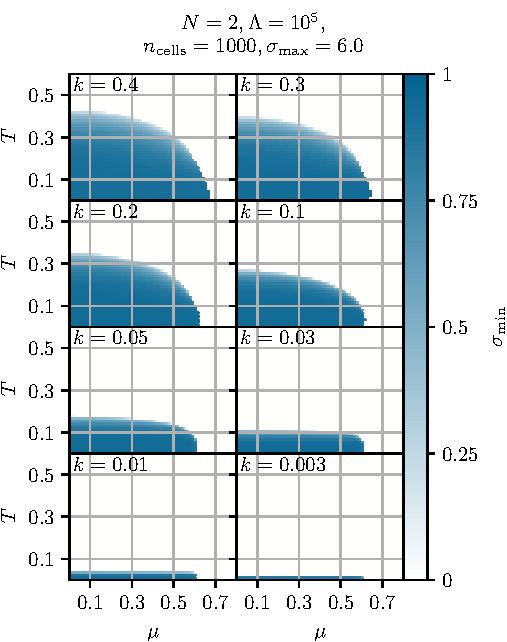
\includegraphics[width=\subcaptionFigureWidth]{gn/figures/phase_diagram.pdf}% Figure (a)
		\captionsetup{font=footnotesize,width=\subcaptionFigureWidth}%
		\caption{
			Density plots of $\sigma_\mathrm{min}(t)$.
			Considering the color gradient across the transition line, the order of the phase transition is inferable.
		}% Caption (a)
		\label{fig:phase_diagram}% label (a)
	}
	{%
		Phase diagram of the \gnym{} in the $\mu$-$T$-plane with $N = 2$ at selected \rgscales{} $k ( t )$ during the \frg{} flow, where condensation is present. 
		Phase transition lines on the left \subref{fig:phase_boundaries} and corresponding density plots on the right \subref{fig:phase_diagram}.
		The plots are extracted from $3432$ independent \frg{} flows at points $( \mu_i, T_j )$ with $\mu_i = 0.0125 \cdot i$, $i \in \{ 0, \ldots, 65 \}$ and $T_j = 0.0125 \cdot j$, $j \in \{ 1, \ldots, 48 \}$. For better resolution at small temperatures, we also included calculations at points with $T_j = 0.00625 \cdot j$, $j \in \{ 1, \ldots, 4 \}$ and the same $\mu_i$ as before.
		\fromFigs{19 and 20}{Stoll:2021ori}
	}% Caption
	{fig:finiteNpd}% Label
	
	With this subsubsection we finally turn to a discussion of the phase diagram in the $\mu$-$T$-plane at finite $N$. We focus explicitly on $N = 2$ but the qualitative statements should, following \cref{subsubsec:variableN}, generalize to finite $N > 2$.
	
	In \cref{fig:phase_boundaries} we plot the phase transition lines in the $\mu$-$T$-plane for different $k ( t )$.
	For slightly larger and smaller values of $k ( t )$ \dash{} including the physical point in the \ir{} \dash{} than those that are presented, there is no phase with \ZII{} symmetry breaking at finite temperature. 
	For $k(t)>0.4$ not enough momentum modes are included to allow for the formation of a non-trivial minimum by fermionic fluctuations, while for scales $k(t)<0.003$ bosonic long-range fluctuations already vaporized the condensate. With \cref{fig:phase_diagram}, we present complementary density plots for the condensate at the selected $k(t)$ of \cref{fig:phase_boundaries}.

	We find that when symmetry breaking sets in, the phase transition line looks similar to its infinite-$N$ counter part (yellow line in  \cref{fig:phase_boundaries}). However, the region of broken \ZII{} symmetry is smaller at its formation at $k(t)\approx0.4$, since thermal bosonic fluctuations work against the symmetry breaking induced by the fermions. As soon as one further decreases $k ( t )$, the symmetry broken regime shrinks drastically. Interestingly, we can observe directly, that for small $T$ and late \rgtimes{} the phase boundary is almost independent of $\mu$. This was already discussed in the previous subsubsections. Ultimately, the entire \ZII{} symmetry broken phase vanishes for $T > 0$, such that plotting a ``phase diagram'' in the $\mu$-$T$-plane at the physical point in the \ir{} is kind of pointless. Still, \cref{fig:finiteNpd} clearly shows the region in the $\mu$-$T$-plane, where the precondensation phenomenon~\cite{Boettcher:2012cm,Boettcher:2012dh,Boettcher:2013kia,Boettcher:2014tfa,Roscher:2015xha,Khan:2015puu} takes place.

	It is also noteworthy, that the time period during the \frg{} flow, hence the range of \rgscales{}, where we find \ZII{} symmetry breaking, is rather small (approximately $k \in [ 0.4, 0.003 ]$ spanning over roughly two orders of magnitude), if compared to the total flow time, respectively the nine-orders of magnitude between the \uv{} scale $k_\mathrm{UV} = \Lambda = 10^5$ and the \ir{} scale $k_\mathrm{IR} = 10^{-4}$. A dynamical range of roughly two orders of magnitude starting at around $k(t)\approx 1$ was also observed in the previous subsubsections for computations at $T>0$ and $N=2$.\bigskip
	
	We conclude this subsubsection with a few remarks regarding the situation at zero temperature and finite $N$. From the $N=2$ computations in vacuum, presented in the previous \cref{subsubsec:vacFiniteN_LD1}, we have strong reasons to believe that \ZII{} symmetry breaking persists in vacuum for finite $N$ at low \rgscales{} in the \ir{}. The results obtained by direct computations at low temperatures and $\mu\geq 0$ discussed in \cref{subsubsec:variableT} support this notion and suggest that \ZII{} symmetry breaking persists at non-zero $\mu$ until a chemical potential of $\mu\approx 0.6$ is reached. For $\mu \smallergtrsim 0.6$ at $T=0$ and $N=2$ we do not expect symmetry breaking in the \ir{}. In order to give a more definite and refined picture of the situation at $T=0$ and $\mu\geq 0$ further computations as well as research and development are required including computations at even lower \rgscales{} as well as direct computations at $T=0$ and $\mu>0$ for finite $N$.
	
	A phase transition at zero temperature driven by an external parameter (or field) rather than thermal fluctuation is called a quantum phase transition~\cite{Sachdev:2011}. In the context of the \gnyBm{} at zero temperature the chemical potential acts as such an external parameter. Fermionic vacuum fluctuations are responsible for symmetry breaking in vacuum and low $\mu$, while density fluctuations induced by a non-zero chemical potential (at finite and infinite $N$) as well as bosonic quantum fluctuations (at finite $N$ only) drive the system towards symmetry restoration. For a general pedagogic discussion of quantum phase transitions we refer to the textbook~\cite{Sachdev:2011} as well as the review article~\cite{Dutta:2010}. There are multiple systems known to exhibit a quantum phase transition, see, \eg{}, \ccite{Sachdev:2011,Dutta:2010} and references therein.